\section{Studie av konvektionsparametern}

Finita element har använts även för att studera konvektionsparametern. Hastigheterna har alla
sats till noll på randerna med $h=\unit[6,19]{W~m^{-2}~K^{-1}}$ vilket motsvarar en helt vindstilla dag.
Husets tak är adiabadiskt
och problemet är studerat under en natt i jämviktsläge, det vill säga en evig natt, med
$T_\text{ref} = \unit[0]{^\circ C}$ som referenstemperatur och $T_\text{inne} = \unit[20]{^\circ C}$ inomhus.
Väggens U-värde är satt till $U = \unit[1,19]{W~m^{-2}~K^{-1}}$ vilket motsvarar den oisolerade söderväggen på fastigheten på Walleriusgatan. Penaltyparametern är satt till $\lambda = \unit[10^7]{Pa~s}$.

\begin{figure}
\centering
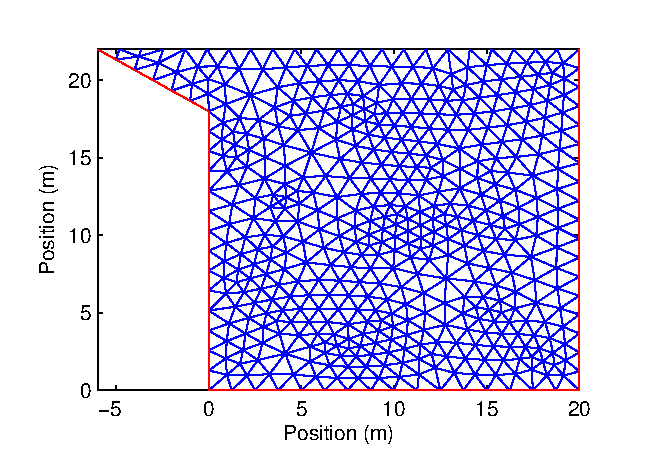
\includegraphics{images/triconvec.eps}
\caption{Definitionsmängd samt triangulering av problemuppställningen för studie av konvektion.}
\end{figure}

Svartkroppsstrålningen approximeras med första ordningens taylorutveckling och
för varje steg löses det slutgiltiga ekvationssystemet med den
modifierade Newton-Raphsons metod. När systemet har lösts beräknas
medeltemperaturen på väggen. Denna används sedan som gissning och utvecklingspunkt
för ovan nämnda taylorutveckling. Denna process upprepas tills medeltemperaturen
ligger tillräckligt nära gissningen. Således genomförs en rad newtonsteg
för att bestämma strålningseffekten från fastigheten genom svartkroppsstrålning.

Sist beräknas konvektionsparametern då mängden energi som transporteras
genom luften är känd. I jämvikt gäller

\begin{equation}
\label{eq:convectionmethod:balance}
Q_\text{vägg} + Q_\text{svartkropp} = Q_\text{konvektion}
\end{equation}

Här är $Q_\text{vägg}$ energin som flödar genom väggen, $Q_\text{svartkropp}$ är energin från
svartkroppsstrålning och $Q_\text{konvektion}$ är då energin som transporteras med konvektion
för att jämvikt skall uppstå.

Medeltemperaturen $\bar{T}$ på väggen och referenstemperaturen $T_\infty$ är kända
vilket ger att h-värdet kan beräknas enligt

\begin{align}
Q_\text{konvektion} &= h(\bar{T}-T_\infty) \Rightarrow \nonumber \\
h &= \frac{Q_\text{vägg} + Q_\text{svartkropp}}{\bar{T}-T_\infty}
\end{align}


\begin{figure}[hpbt]
\centering
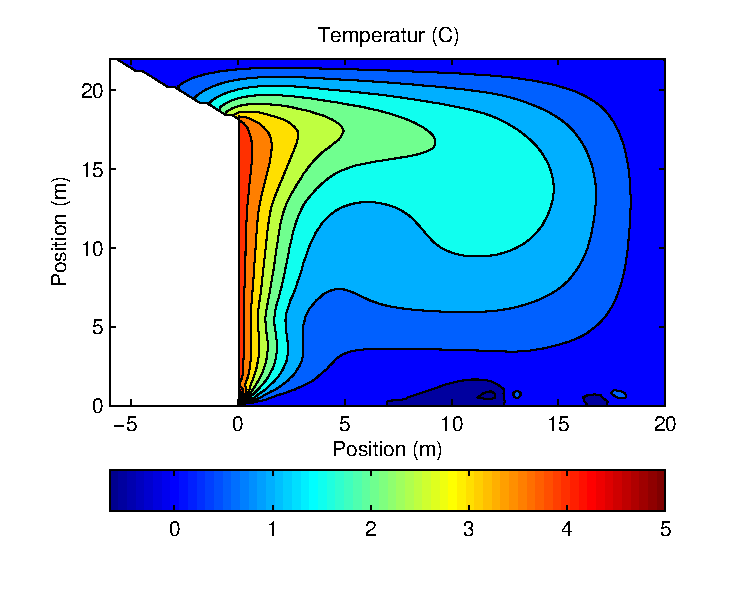
\includegraphics[width=10cm]{images/convectemperature.eps}
\caption{\label{fig:temp_dist}Temperaturfördelningen i $^\circ\mbox{C}$ utanför en vägg, beräknad med finita element av penalty-metoden. Inomhus\-tempertur $\unit[20]{^\circ C}$, utomhustemperatur $\unit[0]{^\circ C}$.}
\end{figure}

% RESULTAT                                                                                                                                    
Denna metod har slutligen verifierats. Som kan ses i figuren~\ref{fig:temp_dist} är luften närmast väggen upp till fem grader 
högre än omgivningen. När det blåser försvinner den här temperaturskillnaden. Detta
visar tydligt hur viktigt det är att inte bara reglera efter utomhustemperaturen.
Här finns dock anomala temperaturer vid nedre randen. Detta tyder på problem med
metodiken.
%%%%%%%%%%%%%%%%%%%%%%%%%%%%%%%%%%%%%%%%%%%%                                                                                                  
Även hastighetsfältet för temperaturens flöde då det är vindstilla har beräknats med finita element metoden
applicerad på penalty-metoden. Detta kan ses i figur~\ref{fig:velocityfield} där också
beloppet av hastighetsfältet visas och det kan noteras att hastigheterna orimligt små.

\begin{figure}[hpbt]
\begin{center}
\subfloat[Hastighetsfält]{
\raisebox{1.2cm}
	{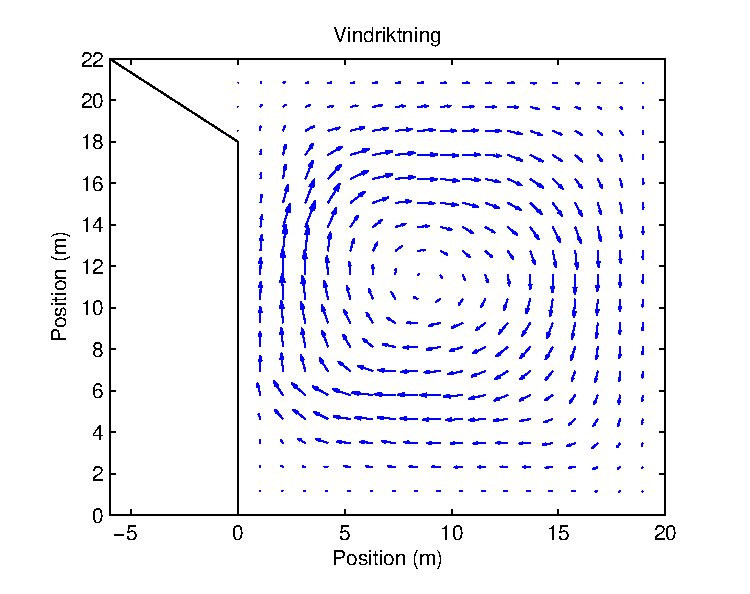
\includegraphics[height=4.9cm]{images/convecquiver.eps}
}}
\subfloat[Beloppet av hastigheten]{
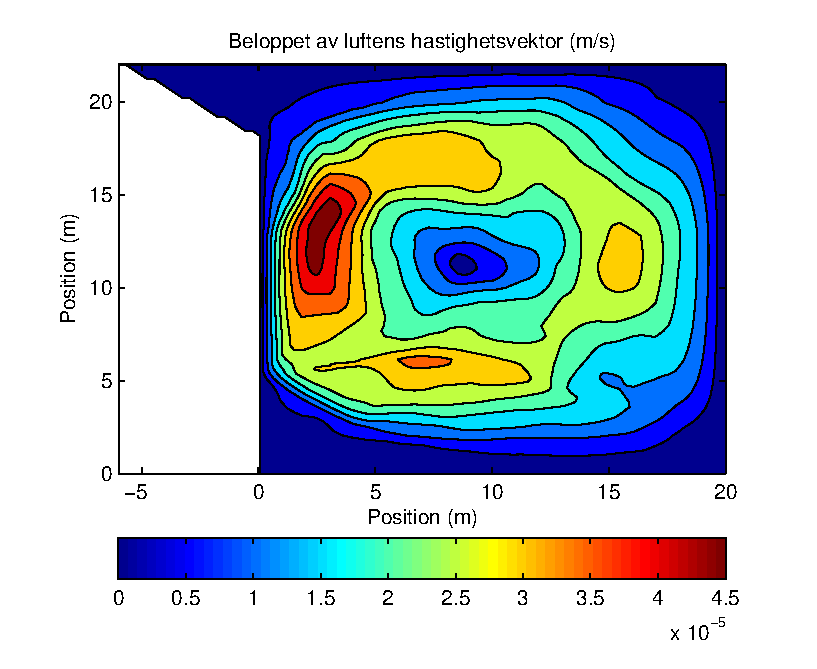
\includegraphics[height=6.2cm]{images/convecspeed.eps}
}
\caption{\label{fig:velocityfield} Hur luften vid husväggen flödar vid en temperaturskillnad.}
\end{center}
\end{figure}


Då sedan konvektionsparametern beräknas utifrån detta blir den väldigt liten,
se figur~\ref{fig:konv_param}. Tyvärr verkade det inte som att metodiken som användes
för att framställa ovanstående data fungerade tillräckligt bra för att med någon
noggrannhet studera fenomenet konvektion. Vi menar dock att formen på hastighetsflödet intill marken och väggen
kan anses vara av rätt karaktär och visar på hur luften rör sig vid husväggen. Randerna mot
luft kan påverka då det inte var tillåtet för luften att passera där, vilket också kan vara en felkälla till den absurt låga konvektionsparametern.

\begin{figure}[hpbt]
\centering
\subfloat[\label{fig:h_reftemp}Konvektions\-koefficienten h mot referens\-temperaturen.]{
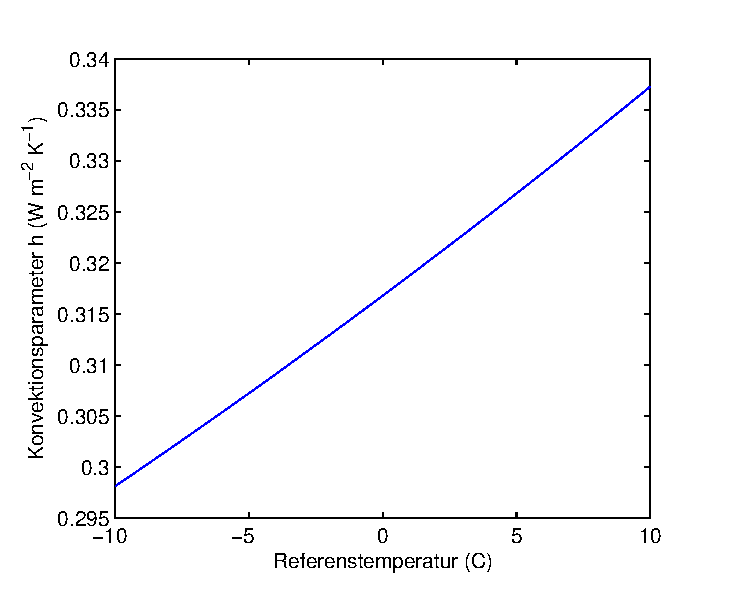
\includegraphics[scale=0.5]{images/convech.eps}
}
\subfloat[\label{fig:h_penalty}Konvektions\-koefficienten h mot penalty\-parametern.]{
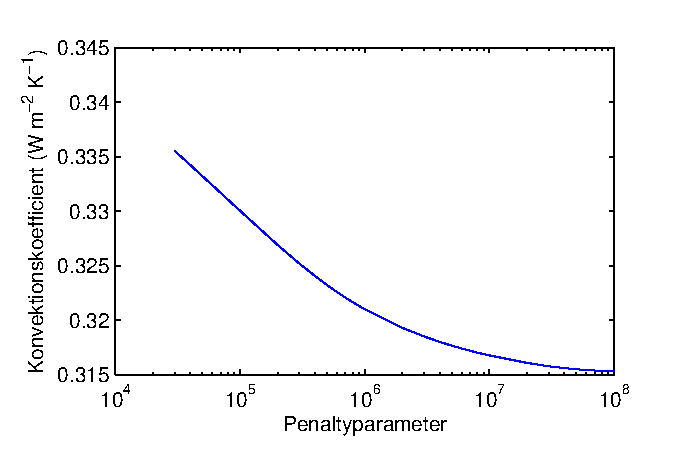
\includegraphics[scale=0.5]{images/convecpenalty.eps}
}\vspace{1cm}

\subfloat[\label{fig:h_volexp}Konvektions\-koefficienten h mot den volymetriska expansions\-koefficienten.]{
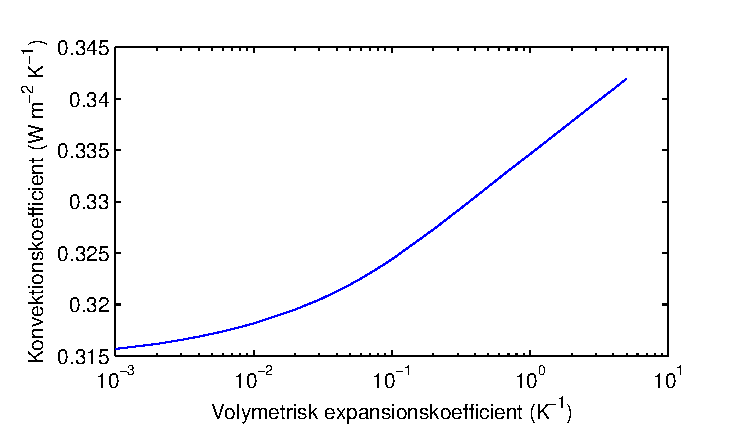
\includegraphics[scale=0.5]{images/convecbeta.eps}
}

\caption{\label{fig:konv_param}Stabilitets\-beräkningar av konvektions\-koefficienten h mot några
parametrar och natur\-konstanter i finita element\-simuleringen av Navier-Stokes ekvationer.
Inomhus\-temperaturen är satt konstant till $\unit[20]{^\circ C}$ med en vägg vars U-värde är
$\unit[1,19]{ W~m^{-2}~K^{-1}}$. Detta skall motsvara söder\-väggen på fastigheten som detta arbete behandlar.}

\end{figure}

% RESULTAT                                                                                                                                    
I figur~\ref{fig:h_reftemp} har beteendet hos metoden som bygger på finita elementmetoden studerats vid variation på några essentiella storheter i modellen.
Först har penaltyparametern varierats i figur~\ref{fig:h_penalty} och här kan det ses att modellens beteende inte förändras nämnvärt
beroende på val av parameter när denna närmar sig storleksordningen $\lambda = \unit[10^7]{Pa~s^{-1}}$. Det linjära förhållandet mellan
konvektionskoefficienten och temperaturdifferensen är intressant men saknar stöd i litteraturen då den rimligtvis borde vara
konstant eller nästan konstant. Slutligen varieras den volymetriska expansionskoefficienten
i figur~\ref{fig:h_volexp}. Det är denna storhet
som gör att luften stiger när den blir varm och det är av denna anledning fenomenet fri konvektion uppstår. Konvektionskoefficienten
ser ut att öka mer än logaritmiskt men däremot inte så snabbt. Anledningen till att penaltyparametern varierades var för
att studera hur stor den skulle behöva bli innan konvektionen började få samma energitransporterande egenskaper
som den förväntats ha. Som kan ses så kommer inte modellen ens i närheten av förväntat värde, inte ens då volymetrisk expansionskoefficient ett mycket högt värde.

Slutligen kan vi bara konstatera att det inte gick att använda denna metod för att studera konvektionsparametern $h$. Litteraturen
som ligger till grund för detta har använt sig av Streamline-Upwind/Petrov-Galerkin (SUPG)\cite{heinrich88}\cite{roy05}. Ovanstående metod är dock
Standard Galerkin med linjära triangulära element. Det är känt att Standard Galerkin kan leda till korsvindsproblem och lösningar som inte är
exakta och stabila\cite{segal2011}.
En misstanke är att det är detta problem vi ser även om detta inte verifieras genom att studera hastighetsfältet. Andra
möjliga orsaker kan vara randvillkor, för liten vald definitionsmängd eller något fel i den matematiska beskrivningen alternativt
vid implementeringen i Matlab.
